

%---------------------------------------------------------------------------%
\frame{
\frametitle{Continuous Uniform Distribution}
A random variable X is called a continuous uniform random variable over the interval $(a,b)$ if it's probability density function is given by
\[ f_{X}(x) = { 1 \over b-a} \hspace{1cm} \mbox{ when } a \leq x \leq b \mbox{     (otherwise } f_X(x) = 0 ) \]
The corresponding cumulative density function is
\[ F_x(x) = { x-a \over b-a} \hspace{1cm} \mbox{ when } a \leq x \leq b\]
}
%----------------------------------------------------------------------------------------------------%
\begin{frame}
\frametitle{The Continuous Uniform Distribution}

\vspace{-0.5cm}

\begin{center}
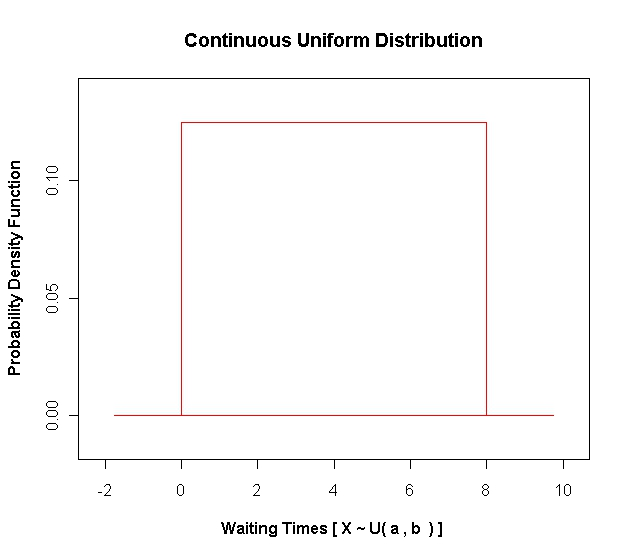
\includegraphics[scale=0.35]{6AUniform}

\end{center}
\end{frame}
%---------------------------------------------------------------------------%
\frame{
\frametitle{Continuous Uniform Distribution}
\begin{itemize}
\item The continuous distribution is very simple to understand and implement, and is commonly used in computer applications (e.g. computer simulation).
\item It is also known as the `Rectangle Distribution' for obvious reasons.
\item We specify the word ``continuous" so as to distinguish it from it's discrete equivalent: the discrete uniform distribution.
\item Remark; the dice distribution is a discrete distribution with lower and upper limits 1 and 6 respectively.
\end{itemize}
}

\frame{
\frametitle{Uniform DistributionParameters}


The continuous uniform distribution is characterized by the following parameters

\begin{itemize}
\item The lower limit $a$
\item The upper limit $b$
\item We denote a uniform random variable $X$ as $X \sim U(a,b)$
\end{itemize}

It is not possible to have an outcome that is lower than $a$ or larger than $b$.

\[ P(X < a) = P(X > b) = 0\]
}

%------------------------------------------------------------------------%
\frame{\frametitle{Interval Probability}

\begin{itemize}
\item We wish to compute the probability of an outcome being within a range of values.
\item We shall call this lower bound of this range $L$ and the upper bound $ U$.
\item Necessarily $L$ and $U$ must be possible outcomes.
\item The probability of $X$ being between $L$ and $U$ is denoted $P( L \leq X \leq U )$.

\[
P( L \leq X \leq U ) = { U - L \over b - a}
\]
\item (This equation is based on a definite integral).
\end{itemize}
}
%---------------------------------------------------------------------------------------------------------%
\frame{
\frametitle{Uniform Distribution: Cumulative Distribution}
\begin{itemize}

\item For any value ``c" between the minimum value a and the maximum
value $b$, we can say
\item $P(X \geq c)$ \[P(X \geq c) = {b-c \over b-a}\]
here $b$ is the upper bound while $c$ is the lower bound
\item $P(X \leq c)$ \[P(X \leq c) = {c-a \over b-a}\]
here $c$ is the upper bound while $a$ is the lower bound.
\end{itemize}
}

%-----------------------------------------------------------------------------%
\frame{
\frametitle{Uniform Distribution: Mean and Variance}
\begin{itemize}
\item The mean of the continuous uniform distribution, with parameters $a$ and $b$ is
\[ E(X) = {a+b \over 2}\]
\item The variance is computed as
\[ V(X) = {(b-a)^2 \over 12}\]
\end{itemize}
}
%------------------------------------------------------------------------%
\frame{
\frametitle{Uniform Distribution: Example}

\begin{itemize}
\item Suppose there is a platform in a subway station in a large large city. \item Subway trains arrive \textbf{every three minutes} at this platform. \item What is the shortest possible time a passenger would have to wait for a train?
\item What is the longest possible time a passenger will have to wait?
\end{itemize}

}


%------------------------------------------------------------------------%
\frame{
\frametitle{Uniform Distribution: Example}

\begin{itemize}
 \item What is the shortest possible time a passenger would have to wait for a train?
%\begin{itemize}
\item If the passenger arrives just before the doors close, then the waiting time is zero.
\[ a = 0 \mbox{ minutes } \]
\end{itemize}
}


%------------------------------------------------------------------------%
\frame{
\frametitle{Uniform Distribution: Example}

\begin{itemize}
\item What is the longest possible time a passenger will have to wait?
%\begin{itemize}
\item If the passenger arrives just after the doors close, and missing the train, then he or she will have to wait the full three minutes for the next one.
\[ b = 3 \mbox{ minutes }  = 180 \mbox{ seconds}  \]
\end{itemize}
%\end{itemize}

}

%------------------------------------------------------------------------%
\frame{
\frametitle{Uniform Distribution: Example}

\begin{itemize}
\item What is the longest probability that he will have to wait longer than 2 minutes?
\[ P(X \geq 2)  = {3-2 \over 3-0} = {1/3} = 0.33333   \]
\end{itemize}
%\end{itemize}

}

%----------------------------------------------------------------------------------------------------%
\begin{frame}
\frametitle{The Continuous Uniform Distribution}

\vspace{-0.5cm}

\begin{center}
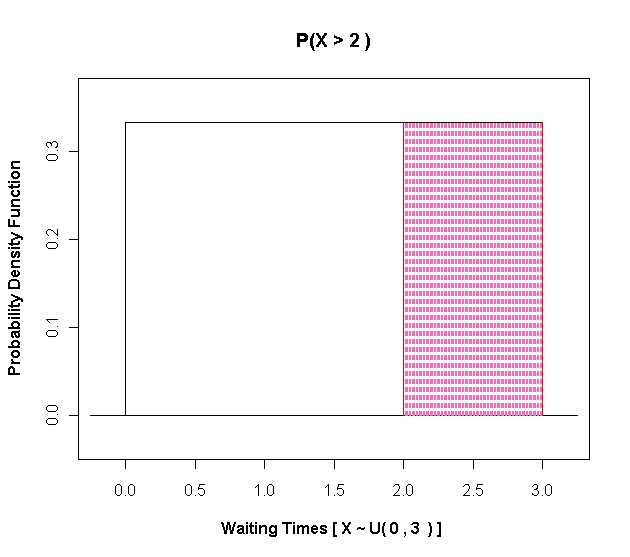
\includegraphics[scale=0.35]{6AUniform4}

\end{center}
\end{frame}
%------------------------------------------------------------------------%
\frame{
\frametitle{Uniform Distribution: Example}

\begin{itemize}
\item What is the longest probability that he will have to wait less than than 45 seconds (i.e. 0.75 minutes)?
\[ P(X \leq 0.75)  = {0.75 - 0 \over 3-0} = {0.75/3} = 0.250  \]
\end{itemize}
%\end{itemize}

}
%----------------------------------------------------------------------------------------------------%
\begin{frame}
\frametitle{The Continuous Uniform Distribution}

\vspace{-0.5cm}

\begin{center}
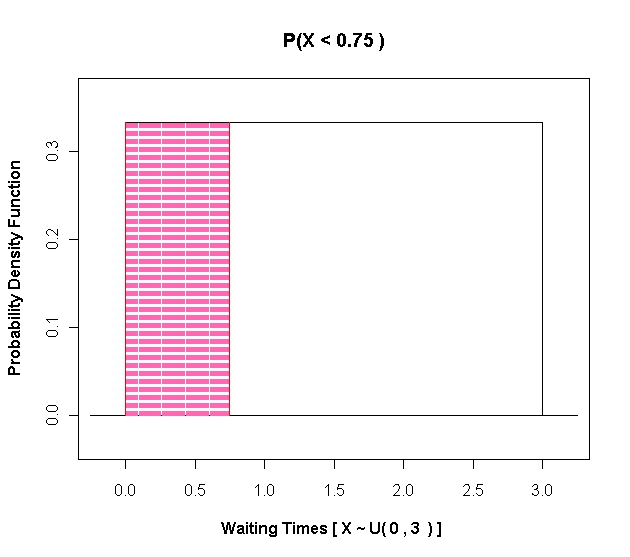
\includegraphics[scale=0.35]{6AUniform3}

\end{center}
\end{frame}
%------------------------------------------------------------------------%
\frame{
\frametitle{Uniform Distribution: Expected Value}

We are told that, for waiting times,  the lower limit $a$ is 0, and the upper limit $b$ is 3 minutes. \\ \bigskip The expected waiting time $\textrm{E}[X]$ is computed as follows
\vspace{0.1cm}
\[
\textrm{E}[X] = {b + a \over 2} =  {3 + 0  \over 2}  = 1.5 \mbox{ minutes }
\]

}
%------------------------------------------------------------------------%
\frame{\frametitle{Uniform Distribution: Variance}

The variance of the continuous uniform distribution, denoted $\textrm{V}[X]$,  is  computed using the following formula
\vspace{0.1cm}
\[
\textrm{V}[X] = {(b - a)^2 \over 12}
\]
\vspace{0.1cm}
For our previous example this is
\[
\textrm{V}[X] = {(3 - 0)^2 \over 12} =  {3^2 \over 12} = {9 \over 12} = 0.75
\]
}




